\documentclass[a4paper,12pt]{article}
\usepackage[utf8]{inputenc}
\usepackage[T1]{fontenc}
\usepackage{amssymb}
\usepackage{amsthm}
\usepackage{amsmath}
\usepackage[english]{babel}
\usepackage{times}
\usepackage{anysize}
\usepackage{titlesec}
\usepackage{fancyhdr}
\usepackage{tikz}
\usepackage{courier}

\usetikzlibrary{positioning}
\tikzset{main node/.style={circle,fill=red!20,draw,minimum size=1cm,inner sep=0pt},}
\tikzstyle{ann} = [fill=lime,font=\footnotesize,inner sep=1pt]

\newcommand\tab[1][0.4cm]{\hspace*{#1}}

\usepgflibrary{arrows}

\setcounter{section}{14}
\setcounter{footnote}{16}
\setcounter{subsection}{1}
\setcounter{figure}{29}
\setcounter{page}{111}
\setcounter{equation}{9}

\pagestyle{fancy}
\fancyhf{}
\lhead{\ref{r15} \tab ŚRODOWISKO MATEMATYCZNE I GRAFY}
\renewcommand{\footrulewidth}{0.4pt}
\rfoot{Strona \thepage}
\cfoot{***}

\begin{document}
    \section{Środowisko matematyczne i grafy}
    \label{r15}
        \subsection{Instrukcja}

        Należy napisać document klasy $article$, który będzie miał postać taką jak Pani/Pan trzyma w ręku.
        Dopuszczalne są odstępstwa tworzonego przez Panią/Pana dokumentu od tej (papierowej) postaci. Obejmują
        one pewne rozszerzenia -- od wersji czarno-białej do kolorowej -- oraz zawężenia do uproszczonej postaci (za dodatkowe "dodatnie" i "ujemne punkty"). Informacje o tych modyfikacjach znajdują sie w przypisach\footnote{To jest pierwszy przypis. Zalecana klasa dokumentu to article z parametrami $a4paper,11pt$}.

        Ta strona zawiera rozdział (\ref{r15}), a w nim dwa podrozdziały\footnote{
        Najlepiej byłoby nadać numer rozdziału ustawiając odpowiedni licznik. W przypadku numerowania innych obiektów -- podobnie, ale należy traktować to jako kosmetykę. Ważniejsze jest, aby w odwołaniach do obiektów używać przypisanych im etykiet.
        }. Wersję źródłową (.tex) i wynikową (.pdf) proszę wysłać na adres \texttt{miller@agh.edu.pl}.

        \subsection{Zadania}
        \begin{enumerate}
            \item Wzór (\ref{10}) pozostawiamy bez interpretacji.

            \begin{equation}
            \label{10}
                \frac{dW}{d\omega dV dt} \simeq
                \begin{cases}
                    \frac{16n_en_iZ^2e^6}{3\sqrt{3}c^3m^2v}g_{ff} & dla \hspace{0.2cm} \text{$\omega \ll \frac{mv^2}{h}$}\\
                    \hspace{2cm} 0 & dla \hspace{0.2cm} \text{$\omega \gg d(a+\frac{mv^2}{h})$}
                \end{cases}
            \end{equation}

            Tu kończy się zadanie pierwsze.

            \item Na rysunku \ref{lab30} jest przedstawiony prosty graf\footnote{
                Zalecany pakiet: $tikz$. Dobrze byłoby odtworzyć kształt łuków (krawędzi grafu). Rozszezenia: wypełnić węzły kolorem jasnoczerwonym, łuki np. niebieskie, opisy łuwków na jasnozielonym tle. Możliwe uproszczenie: wszystkie łuki można narysować linią ciągłą jednakowej grubości.
            }.

            \begin{figure}[!htb]
                \caption{Graf arytmetyczny}
                \label{lab30}
                \centerline{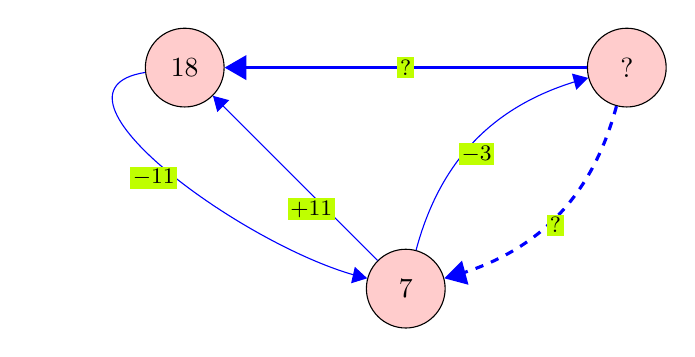
\begin{tikzpicture}[scale=1,inner sep=0.4mm]
                    \node[main node] (2) [left = 2.3cm]  {$18$};
                    \node[main node] (3) [right = 2.3cm] {$?$};
                    \node[main node] (1) [below = 2.3cm] {$7$};
                    \draw[blue, -triangle 60, line width=0.4mm]
                        (3) edge (2);
                    \draw[blue, -triangle 60, bend right, out=-4.5cm]
                        (2) edge (1);
                    \draw[blue, -triangle 60]
                        (1) edge (2) (1) edge [bend left] (3);
                    \draw[blue, -triangle 60]
                        (3) [dashed, bend left, line width=0.4mm] edge (1);
                    \node[ann] at (0,0) {$?$};
                    \node[ann] at (-1.2cm,-1.8cm) {$+11$};
                    \node[ann] at (0.9cm,-1.1cm) {$-3$};
                    \node[ann] at (1.9cm,-2cm) {$?$};
                    \node[ann] at (-3.2cm,-1.4cm) {$-11$};
                \end{tikzpicture}}
            \end{figure}
        \end{enumerate}

        To jest koniec sprawdzianu. Jeżeli jest jeszcze czas, to proszę sprawdzić wszystkie szczegóły\footnote{
            Możliwe uproszczenie: W tym wypunktowaniu można zastąpić znaki $+$ standardową kropką.
        }, np.:
        \renewcommand{\labelitemi}{$+$}
        \begin{itemize}
            \item pozostawianie na końcu linii wyrazów jednoliterowych,
            \item wyrównanie w pionie elementów wyrażeń matematycznych,
            \item postaci paginy dolnej i górnej, numeracji itp.
        \end{itemize}
\end{document}
